\documentclass[tikz,border=5pt]{standalone}
\usepackage[UTF8]{ctex}
\usepackage{amsmath,amssymb}
\usetikzlibrary{arrows.meta,calc,angles,quotes,patterns,decorations.pathmorphing}
\definecolor{field}{HTML}{176B9B}
\definecolor{force}{HTML}{B64B32}
\tikzset{>=Latex,line width=.8pt,every node/.style={font=\small},field/.style={color=field},force/.style={color=force},body/.style={draw=black,fill=blue!5},ghost/.style={dashed,gray},labelbox/.style={fill=white,inner sep=1.2pt}}
\begin{document}
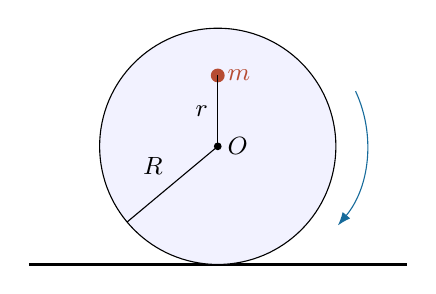
\begin{tikzpicture}
\draw[thick](-2.4,0)--(2.4,0);
\draw[body](0,1.5)circle(1.5);
\fill(0,1.5)circle(1.4pt)node[right]{$O$};
\fill[force](0,2.4)circle(2.5pt)node[right]{$m$};
\draw(0,1.5)--(0,2.4)node[midway,left]{$r$};
\draw(0,1.5)--(-1.15,.54)node[midway,above left]{$R$};
\draw[->,field](1.75,2.2)arc(25:-40:1.6);
\end{tikzpicture}
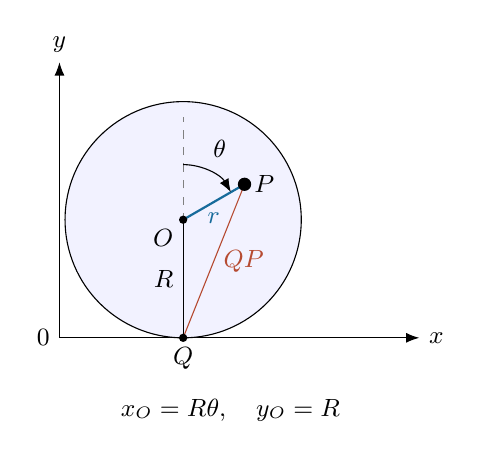
\begin{tikzpicture}
\draw[->](-1.5708,0)--(3,0)node[right]{$x$};
\draw[->](-1.5708,0)--(-1.5708,3.5)node[above]{$y$};
\coordinate(O)at(0,1.5);\coordinate(Q)at(0,0);
\coordinate(P)at(.7794,1.95);\coordinate(U)at(0,2.8);
\draw[body](O)circle(1.5);
\draw[ghost](Q)--(U);
\draw[field,thick](O)--(P)node[midway,below]{$r$};
\draw(O)--(Q)node[midway,left]{$R$};
\draw[force](Q)--(P)node[midway,right]{$QP$};
\draw[->](0,2.2)arc(90:30:.7);
\node[above right]at(.26,2.16){$\theta$};
\fill(O)circle(1.5pt)node[below left]{$O$};
\fill(P)circle(2.4pt)node[right]{$P$};
\fill(Q)circle(1.5pt)node[below]{$Q$};
\node[left]at(-1.5708,0){$0$};
\node[below]at(.6,-.65){$x_O=R\theta,\quad y_O=R$};
\end{tikzpicture}
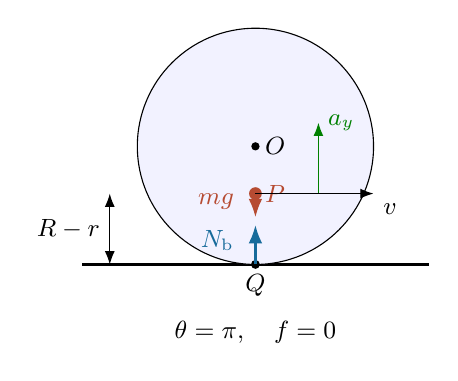
\begin{tikzpicture}
\draw[thick](-2.2,0)--(2.2,0);
\draw[body](0,1.5)circle(1.5);
\fill(0,1.5)circle(1.5pt)node[right]{$O$};
\fill[force](0,.9)circle(2.3pt)node[right]{$P$};
\fill(0,0)circle(1.6pt)node[below]{$Q$};
\draw[field,->,thick](0,0)--(0,.5);
\node[field,left]at(-.15,.3){$N_{\rm b}$};
\draw[force,->,thick](0,.9)--(0,.6);
\node[force,left]at(-.15,.8){$mg$};
\draw[->,green!50!black](.8,.9)--(.8,1.8)node[right]{$a_y$};
\draw[ghost](0,.9)--(.8,.9);
\draw[->](0,.9)--(1.5,.9)node[below right]{$v$};
\draw[<->](-1.85,0)--(-1.85,.9)node[midway,left]{$R-r$};
\node[below]at(0,-.6){$\theta=\pi,\quad f=0$};
\end{tikzpicture}
\begin{tikzpicture}[x=.65cm,y=1.1cm]
\draw[->](-.3,0)--(6.8,0)node[right]{$x/R$};
\draw[->](0,0)--(0,2)node[above]{$y/R$};
\draw[field,thick,domain=0:360,samples=121]plot({\x*pi/180+.5*sin(\x)},{1+.5*cos(\x)});
\foreach\t in{0,180,360}{
\fill({\t*pi/180}, {1+.5*cos(\t)})circle(1.6pt);
}
\foreach\t in{120,240}{
\fill[force]({\t*pi/180+.5*sin(\t)}, {1+.5*cos(\t)})circle(2pt);
}
\node[force,above]at(2.53,.9){$a_n=0$};
\node[below]at(3.1416,0){$\pi$};\node[below]at(6.2832,0){$2\pi$};
\node[left]at(0,.5){$1-k$};\node[left]at(0,1.5){$1+k$};
\node[below]at(3.2,-.65){一个几何周期，$k=1/2$；红点是曲率变号处};
\end{tikzpicture}
\end{document}
